\documentclass[12pt]{article}
\usepackage[utf8]{inputenc}
\usepackage{geometry}
\usepackage{svg}
\usepackage{float}
\usepackage{caption}
\usepackage{amsmath,amsthm,amsfonts,amssymb,amscd}
\usepackage{fancyhdr}
\usepackage{titlesec}
\usepackage{xparse}
\usepackage{listings}
\usepackage{tikz}
\usepackage{mathtools}
\usepackage[ngerman]{babel}
\usetikzlibrary{shapes.geometric, arrows}
\pagestyle{empty}
\titleformat*{\section}{\large\bfseries}

%
\geometry{
 a4paper,
 total={170mm,240mm},
 left=20mm,
 top=30mm,
 }

\date{}
%Bitte ausfüllen
\newcommand\course{Programmierung, Gruppe 16}
\newcommand\hwnumber{4}
\newcommand\Name{Maximilian Petri, 405602}
\newcommand\Neptun{Danje Petersen, 379748}

%Matheinheiten
\newcommand\m{\:\textrm{m}}
\newcommand\M{\:\Big[\textrm{m}\Big]}
\newcommand\mm{\:\textrm{mm}}
\newcommand\MM{\:\Big[\textrm{mm}\Big]}
\newcommand\un{\underline}
\newcommand\s{\:\textrm{s}}
\newcommand\bS{\:\Big[\textrm{S}\Big]}
\newcommand\ms{\:\frac{\textrm{m}}{\textrm{s}}}
\newcommand\MS{\:\Big[\frac{\textrm{m}}{\textrm{s}}\Big]}
\newcommand\mss{\:\frac{\textrm{m}}{\textrm{s}^2}}
\newcommand\MSS{\:\Big[\frac{\textrm{m}}{\textrm{s}^2}\Big]}
\DeclarePairedDelimiter\ceil{\lceil}{\rceil}
\DeclarePairedDelimiter\floor{\lfloor}{\rfloor}

%Einstellungen für lstlisting
\lstset{
basicstyle=\fontsize{9}{10}\selectfont\ttfamily, 
keywordstyle=\color{purple}\bfseries,           % keywords purple
commentstyle=\color{gray},                     % white comments
stringstyle=\color{blue},                       % strings blue
showstringspaces=false,
language= java}                          % typewriter type for strings                       


%Bitte nicht einstellen

\renewcommand{\thesection}{Aufgabe }
\renewcommand{\thesubsection}{\alph{subsection})}
\renewcommand{\thesubsubsection}{\hspace{0.8cm}\roman{subsubsection})}
\renewcommand{\figurename}{Abbildung}
\renewcommand{\tablename}{Tabelle}
\pagestyle{fancyplain}
\headheight 35pt
\lhead{\Name\\\Neptun}
\chead{\textbf{\Large Hausaufgabe \hwnumber}}
\rhead{\course \\ \today}
\lfoot{}
\cfoot{}
\rfoot{\small\thepage}
\headsep 1.5em

\begin{document}

\section{2)}
\subsection{}
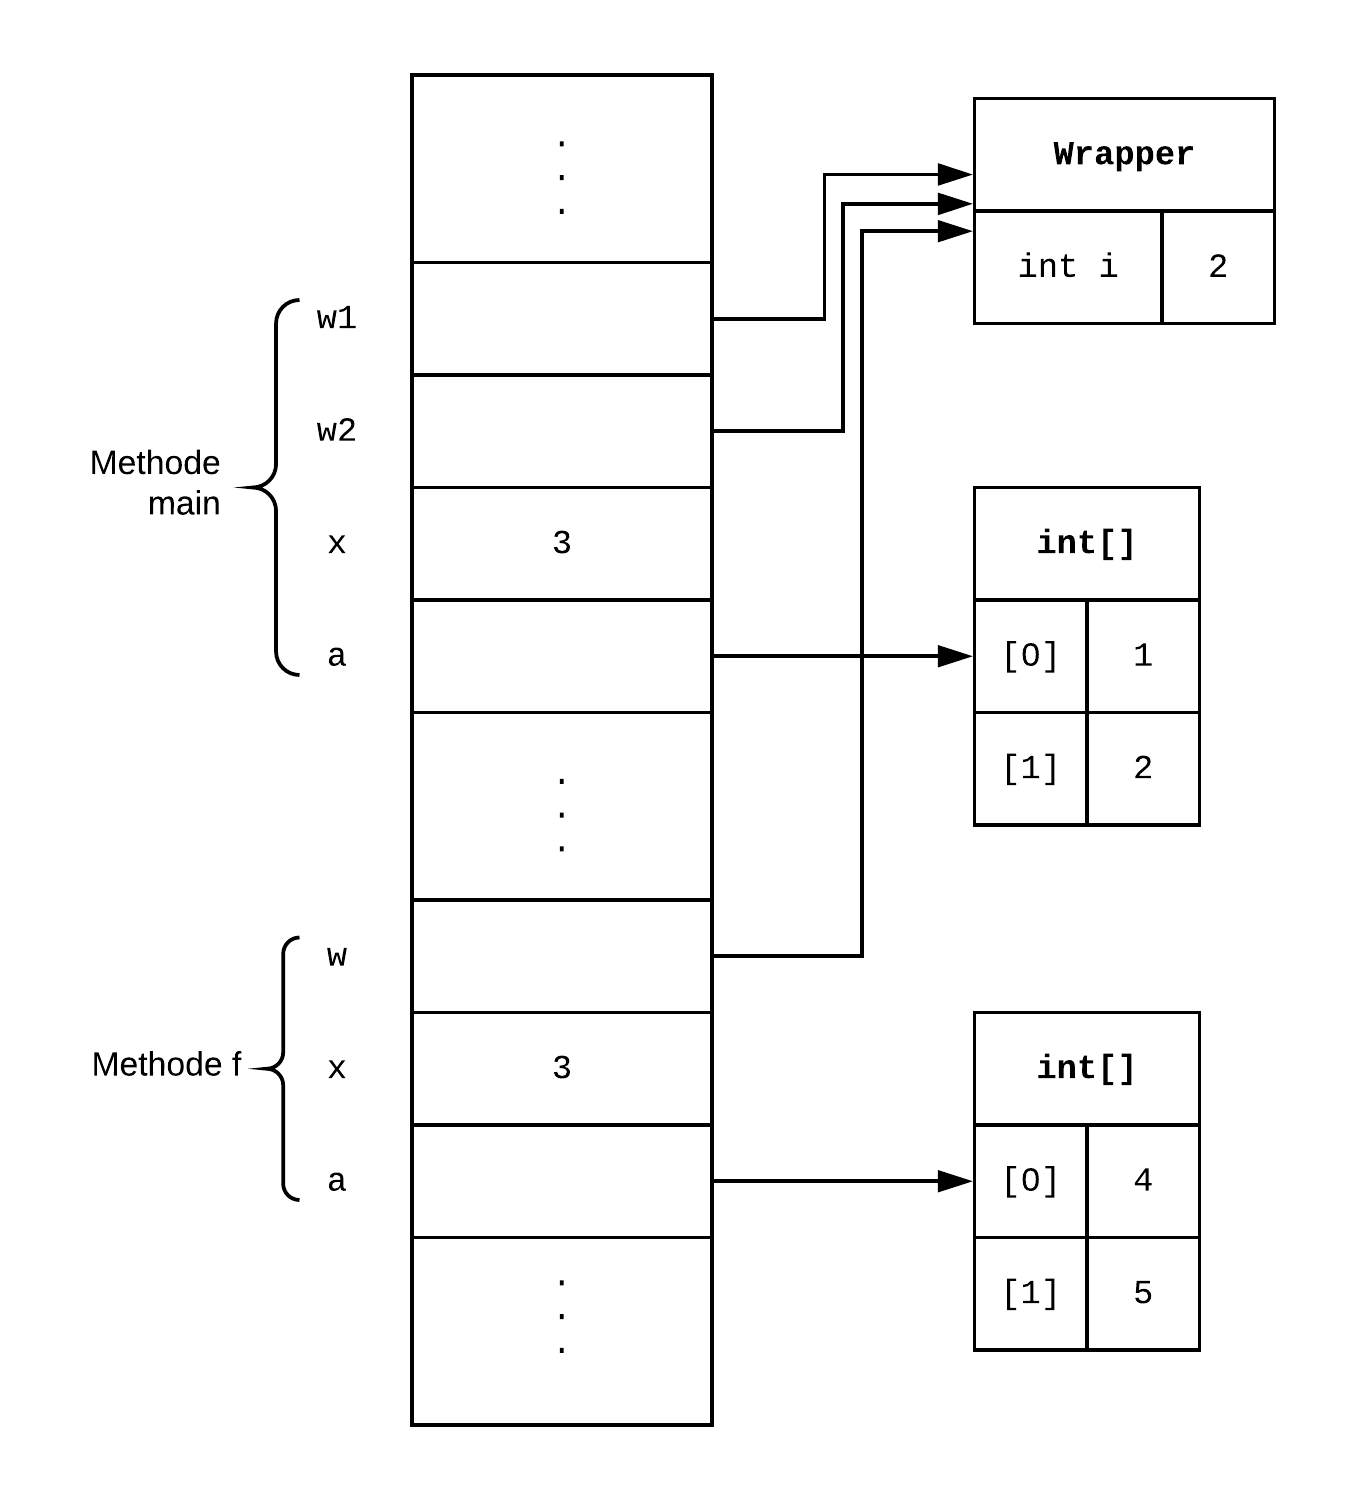
\includegraphics[width=0.6\textwidth]{Speicherstand1.png}

\subsection{}
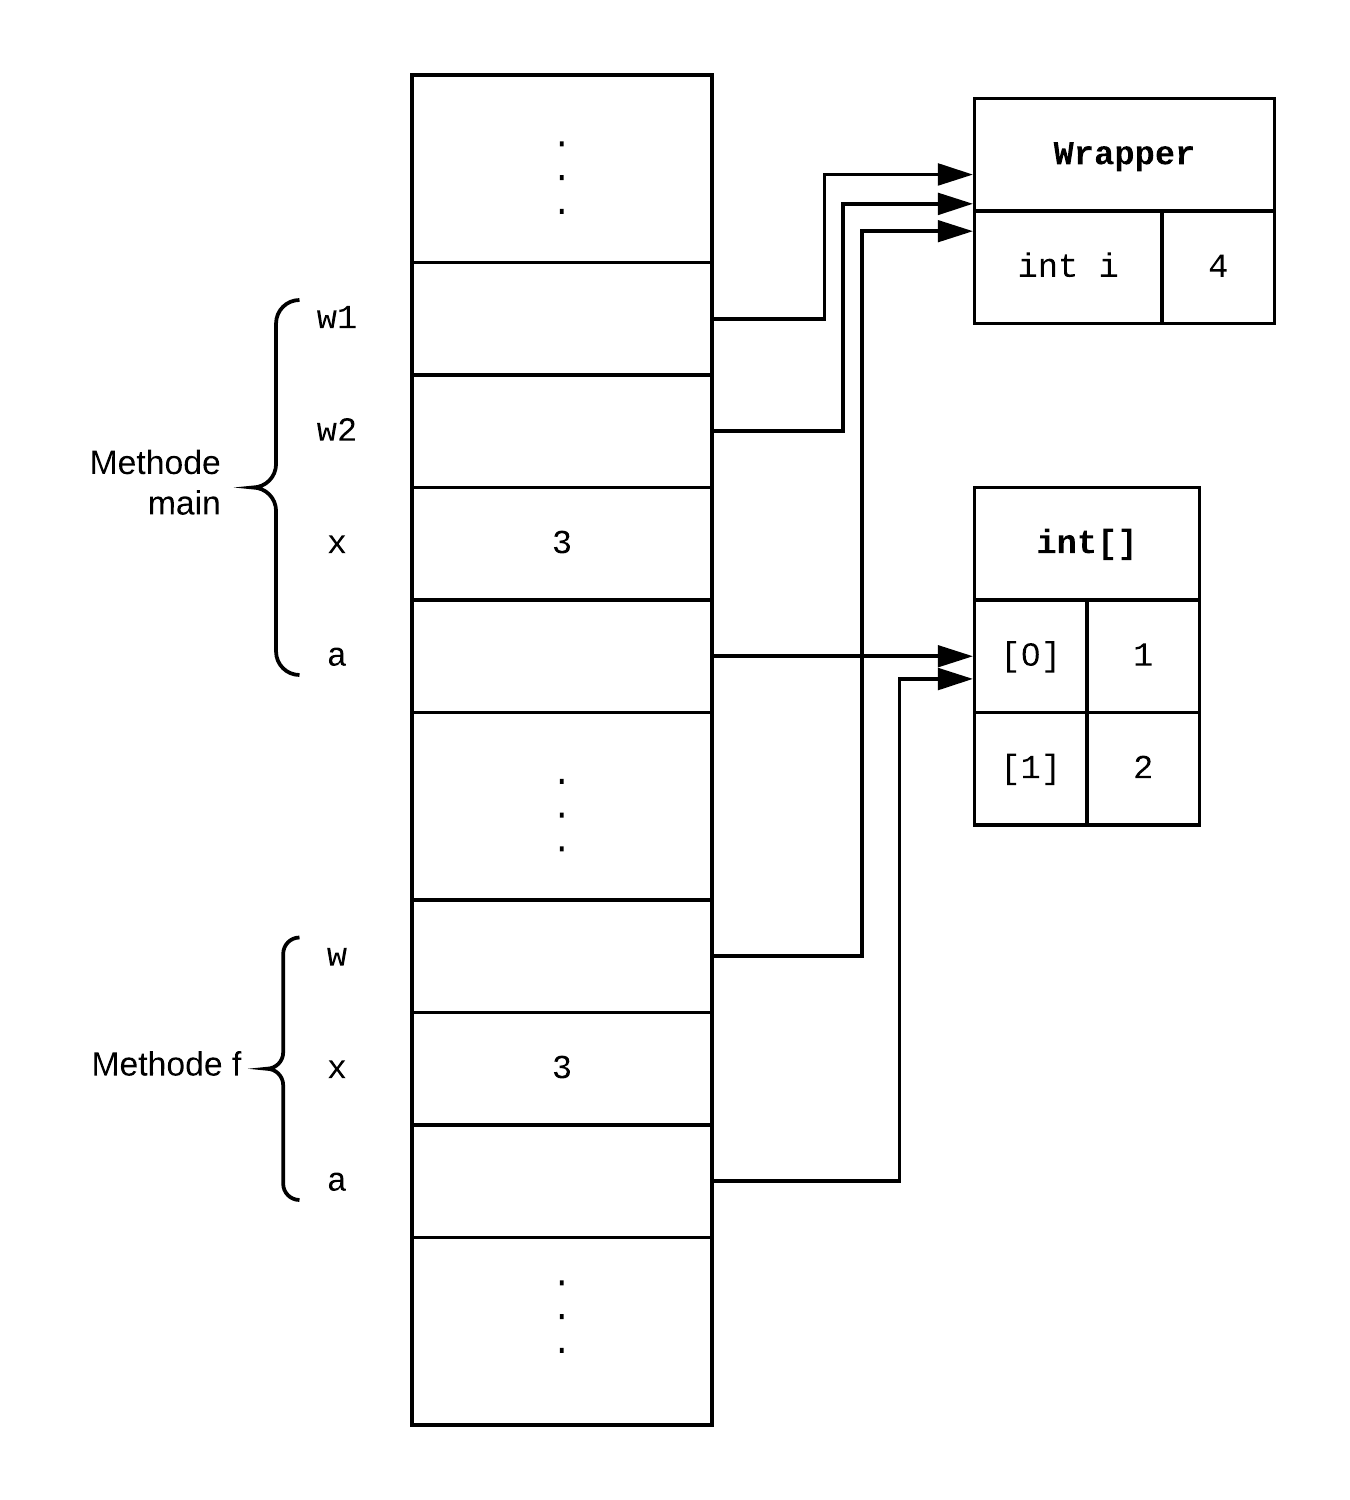
\includegraphics[width=0.6\textwidth]{Speicherstand2.png}

\subsection{}
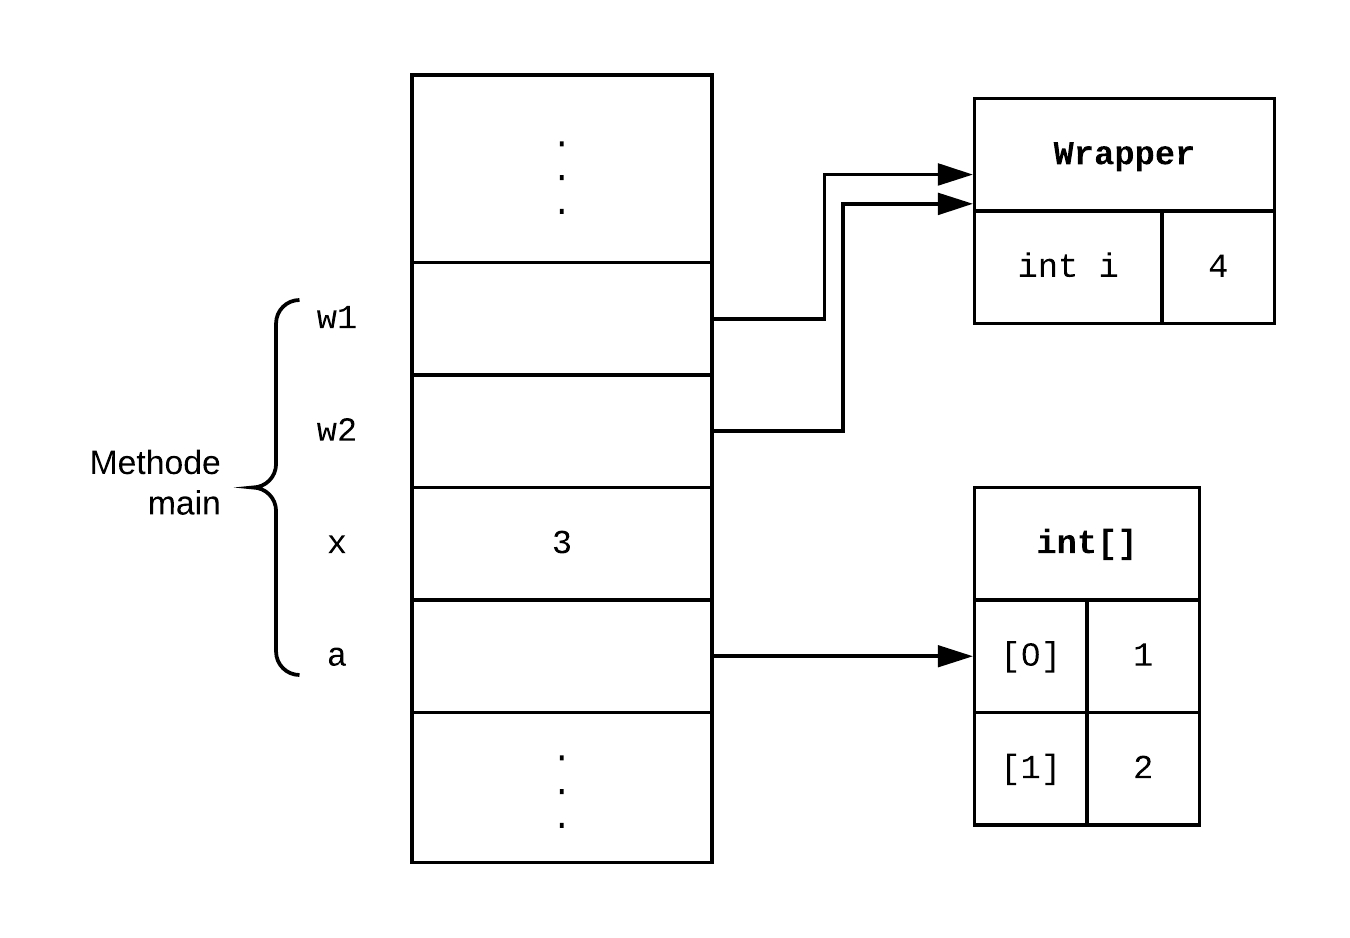
\includegraphics[width=0.6\textwidth]{Speicherstand3.png}
\pagebreak


\section{4)}
\begin{lstlisting}
public class Vector {

    private double[] components;

    public static void main(String[] args) {
        // Set Dimemsion of v1 and v2
        int dim = SimpleIO.getInt("Geben Sie die Dimension der Vektoren ein:");
        Vector v1 = Vector.newWithDimension(dim);
        Vector v2 = Vector.newWithDimension(dim);

        // Set the components of v1 and v2
        SimpleIO.output("Geben Sie die Komponenten des ersten Vektors ein:");
        v1.readComponentsFromUserInput();
        SimpleIO.output("Geben Sie die Komponenten des zweiten Vektors ein:");
        v2.readComponentsFromUserInput();

        // Calculate and output the scalarproduct of v1 and v2
        SimpleIO.output("Das Skalarprodukt der beiden Vektoren ist: " + v1.scalarproduct(v2));
    }

    public static Vector newWithDimension(int n) {
        Vector v = new Vector();
        v.initComponents(n);
        return v;
    }

    public double scalarproduct(Vector q) {
        // check if same length
        if (this.getLength() != q.getLength()) {
            return 0;
        }

        // calculate and return scalaproduct
        double scalarproduct = 0;
        for (int i = 0; i < this.getLength(); i++) {
            scalarproduct += this.getComponent(i) * q.getComponent(i);
        }
        return scalarproduct;
    }

    public void readComponentsFromUserInput() {
        for (int i = 0; i < this.getLength(); i++) {
            components[i] = SimpleIO.getDouble("Geben sie die "
                                                + (i + 1) + "-te Komponente ein:");
        }
    }

    public void initComponents(int n) {
        components = new double[n];
    }

    public int getLength() {
        return components.length;
    }

    public void setComponent(double val, int i) {
        components[i] = val;
    }

    public double getComponent(int i) {
        return components[i];
    }
}
\end{lstlisting}

\end{document}